\chapter{空间中的直线和平面}
\section{平面的方程}\index{PMFC@平面方程}
\subsection{确定平面的条件}
\thispagestyle{empty}
\begin{enumerate}[$\bullet$]
	\setlength{\itemindent}{3em}
	\setlength{\topsep}{0.01em}
	\setlength{\itemsep}{0.01em}
	\item 不在一条直线上的三点确定个平面 .如图\ref{pm1}.
	\item 过一定点且垂直于线可以作个平面.如图\ref{pm2}.
	\item 一条直线和外点确定个平面.如图\ref{pm3}.
	\item 两相交直线确定一个平面.如图\ref{pm4}.
	\item 两平行直线确定一个面.如图\ref{pm5}.
\end{enumerate}
\begin{figure}[h]
	\subfigure[三点]{
		\begin{minipage}[b]{0.33\linewidth}
			\centering
			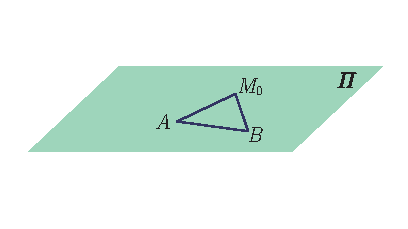
\includegraphics[width=0.9\linewidth]{picture/C-2/2.1/pm1.eps}
			%\caption{fig1}
			\label{pm1}
		\end{minipage}%
	}%
	\subfigure[定点加垂线]{
		\begin{minipage}[b]{0.33\linewidth}
			\centering
			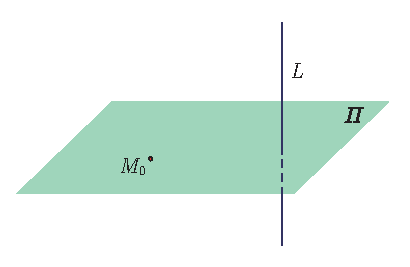
\includegraphics[width=0.9\linewidth]{picture/C-2/2.1/pm2.eps}
			%\caption{fig2}
			\label{pm2}
		\end{minipage}%
	}%
	\subfigure[外点加直线]{
		\begin{minipage}[b]{0.33\linewidth}
			\centering
			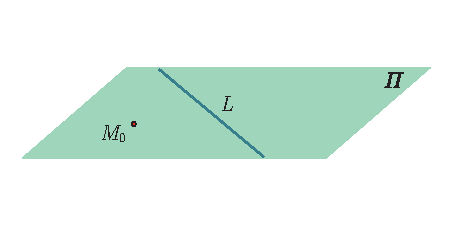
\includegraphics[width=0.95\linewidth]{picture/C-2/2.1/pm3.eps}
			%\caption{fig2}
			\label{pm3}
		\end{minipage}%
	}%
	
	\subfigure[两相交直线]{
		\begin{minipage}[b]{0.5\linewidth}
			\centering
			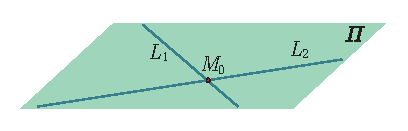
\includegraphics[width=0.9\linewidth]{picture/C-2/2.1/pm4.eps}
			%\caption{fig2}
			\label{pm4}
		\end{minipage}%
	}%
	\subfigure[两平行直线]{
		\begin{minipage}[b]{0.5\linewidth}
			\centering
			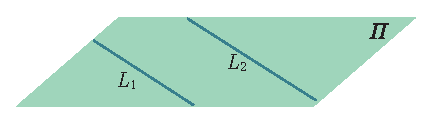
\includegraphics[width=0.9\linewidth]{picture/C-2/2.1/pm5.eps}
			%\caption{fig2}
			\label{pm5}
		\end{minipage}%
	}%
	\centering
	\caption{确定平面的条件}
\end{figure}
\newpage 
\subsection{通用的平面方程}
\begin{enumerate}[\large1.]
	\item {\color{dy}\large 坐标式方程(参数方程\index{PMFC@平面方程!CSFC@参数方程})}\index{PMFC@平面方程!ZBSFC@坐标式方程}
	\begin{enumerate}[]
		\item 已知:{\color{dl}平面上一点}:$M_0(x_0,y_0,z_0)$和平面上的{\color{dl}两个不共线的向量(直线)}:$\overrightarrow{a}=(a_1,a_2,a_3),\overrightarrow{b}=(b_1,b_2,b_3)$.
		\item 原理:三向量共面原理:$\overrightarrow{M_0M}=\lambda \overrightarrow{a}+\mu \overrightarrow{b}$.
		\item 表达式:
		\begin{equation}
		\Pi: \begin{cases}
		x=x_0+\lambda a_1+\mu b_1,\\
		y=y_0+\lambda a_2+\mu b_2,\\
		z=z_0+\lambda a_3+\mu b_3.
		\end{cases}
		\end{equation}
	\end{enumerate}
	\item {\color{dy}\large 向量式方程}\index{PMFC@平面方程!XLSFC@向量式方程}
	\begin{enumerate}[]
		\item 已知:{\color{dl}平面上一点}:$M_0(x_0,y_0,z_0)$和平面上的{\color{dl}两个不共线的向量(直线)}:$\overrightarrow{a}=(a_1,a_2,a_3),\overrightarrow{b}=(b_1,b_2,b_3)$.
		\item 原理:$\overrightarrow{OM}=\overrightarrow{OM_0}+\overrightarrow{M_0M}$,三向量共面原理.记$\overrightarrow{OM}=\overrightarrow{r},\overrightarrow{OM_0}=\overrightarrow{r_0}$.
		\item 表达式:
		\begin{equation}
		\overrightarrow{r}=\overrightarrow{r_0}+\lambda \overrightarrow{a}+\mu \overrightarrow{b}
		\end{equation}
	\end{enumerate}
	\item {\color{dy}\large 行列式方程}\index{PMFC@平面方程!HLSFC@行列式方程}
	\begin{enumerate}[]
		\item 已知:{\color{dl}平面上一点}:$M_0(x_0,y_0,z_0)$和平面上的{\color{dl}两个不共线的向量(直线)}:$\overrightarrow{a}=(a_1,a_2,a_3),\overrightarrow{b}=(b_1,b_2,b_3)$.
		\item 原理:三向量共面:$\overrightarrow{M_0M}\cdot \left( \overrightarrow{a}\times\overrightarrow{b}\right) =0$.
		\item 表达式:
		\begin{equation}
		\begin{array}{|ccc|}
		x-x_0 & y-y_0 & z-z_0 \\
		a_1 & a_2 & a_3 \\
		b_1 & b_2 & b_3
		\end{array}=0
		\label{HLS}
		\end{equation}
	\end{enumerate}
	\item {\color{dy}\large 三点式方程}\index{PMFC@平面方程!SDSFC@三点式方程}
	\begin{enumerate}[]
		\item 已知:{\color{dl}不在一条直线上的三点}:$M_1(x_1,y_1,z_1),M_2(x_2,y_2,z_2),M_3(x_3,y_3,z_3)$
		\item 原理:三向量$\overrightarrow{M_1M},\overrightarrow{M_1M_2},\overrightarrow{M_1M_3},$共面:$\overrightarrow{M_1M} \cdot \left( \overrightarrow{M_1M_2}\times\overrightarrow{M_1M_3}\right) =0$.
		\item 表达式:
		\begin{equation}
		\begin{array}{|ccc|}
		x-x_1 & y-y_1 & z-z_1 \\
		x_2-x_1 & y_2-y_1 & z_2-z_1 \\
		x_3-x_1 & y_3-y_1 & z_3-z_1
		\end{array}=0
		\end{equation}
		或
		\begin{equation}
		\begin{array}{|cccc|}
		x & y & z &1\\
		x_1&y_1 &z_1 & 1\\
		x_2& y_2 & z_2& 1\\
		x_3& y_3 & z_3&1
		\end{array}=0
		\end{equation}
		这个式子可以结合四点共面的式子\eqref{SDGM}结合记忆和理解. 
	\end{enumerate}
	\item {\color{dy}\large 一般式方程}\index{PMFC@平面方程!YBSFC@一般式方程}
	\begin{enumerate}[]
		\item 已知:{\color{dl}平面上一点}:$M_0(x_0,y_0,z_0)$和平面上的{\color{dl}两个不共线的向量(直线)}:$\overrightarrow{a}=(a_1,a_2,a_3),\overrightarrow{b}=(b_1,b_2,b_3)$.
		\item 原理:用行列式的知识按第一行展开式\eqref{HLS}.
		\item 表达式:
		\begin{equation}
		Ax+By+Cz+D=0
		\end{equation}
		其中,
		\begin{equation*}
		A=\begin{array}{|cc|}
		a_2 & a_3 \\
		b_2 & b_3
		\end{array}
		\,,\quad 
		B=\begin{array}{|cc|}
		a_3 & a_1 \\
		b_3 & b_1
		\end{array}
		\,,\quad 
		C=\begin{array}{|cc|}
		a_1 & a_2 \\
		b_1 & b_2
		\end{array}
		\,,\quad 
		D=-(Ax_0+By_0+Cz_0).
		\end{equation*}
		{\color{dy}空间任何一个平面$\Longleftrightarrow x,y,z$的三元一次方程. }
	\end{enumerate}
	
	\enbelowtheorem[向量与平面平行定理]
	\quad 设平面$\pi $的方程为
	\begin{equation*}
	Ax+By+Cz+D=0,
	\end{equation*}
	则向量$\overrightarrow{v}=(X,Y,Z)$平行于平面$\pi $的充要条件为
	\begin{equation*}
	AX+BY+CZ=0
	\end{equation*}
	
	\item {\color{dy}\large 截距式方程}\index{PMFC@平面方程!JJSFC@截距式方程}
	\begin{enumerate}[]
		\item 已知:{\color{dl}与坐标轴相交的三点}:$M_1(a,0,0),M_2(0,b,0),M_3(0,0,c)$
		\item 原理:与三点式相同,只是取与坐标轴相交的三个特殊点. 
		\item 表达式:$M_1(a,0,0),M_2(0,b,0),M_3(0,0,c)$代入三点式方程得:
		\begin{equation*}
		\begin{array}{|ccc|}
		x-a & y & z \\
		-a & b & 0 \\
		-a & 0 & c
		\end{array}=bcx+acy+abz=abc.
		\end{equation*}
		由于$abc \ne 0$,那么上式可写为:
		\begin{equation}
		\frac{x}{a}+\frac{y}{b}+\frac{z}{c}=1.
		\end{equation}
	\end{enumerate}
\end{enumerate}
\subsection{直角坐标系平面方程}
\tdefination[法向量]\index{XL@向量!FXL2@法向量}
在空间中给定一个点$M_0$和一个非零向量$\overrightarrow{n}$,那么通过点$M_0$且与向量$\overrightarrow{n}$垂直的平面是惟一确定的,我们把向量$\overrightarrow{n}$叫做这一个平面的法向量. 

\begin{enumerate}[\large1.]
	\item {\color{dy}\large 点法式方程}\index{PMFC@平面方程!DFSFC@点法式方程}
	\begin{enumerate}[]
		\item 已知:{\color{dl}一个定点}:$M_0(x_0,y_0,z_0)$和{\color{dl}一个法向量}:$\overrightarrow{n}=(A,B,C)$.如图\ref{DFS}.
		\item 原理:法向量的性质,即对于平面任意一点$M(x,y,z)$均有$\overrightarrow{MM_0}\cdot \overrightarrow{n}=0$. 
		\item 表达式:设$M_0,M$的位置矢量分别是$\overrightarrow{r_0},\overrightarrow{r}$.
		\begin{equation}
		\overrightarrow{n}\cdot\left(  \overrightarrow{r}-\overrightarrow{r_0}\right) =0
		\end{equation}
		即
		\begin{equation}
		A(x-x_0)+B(y-y_0)+C(z-z_0)+D=0
		\end{equation}
		\quad 令$D=-(Ax_0+By_0+Cz_0)$,那么上式可以表示成一般式:
		\begin{equation}
		Ax+By+Cz+D=0
		\end{equation}
	\end{enumerate}
	\begin{figure}[h]
		\centering 
		\subfigure[点法式方程]{
			\begin{minipage}[b]{0.5\linewidth}
				\centering
				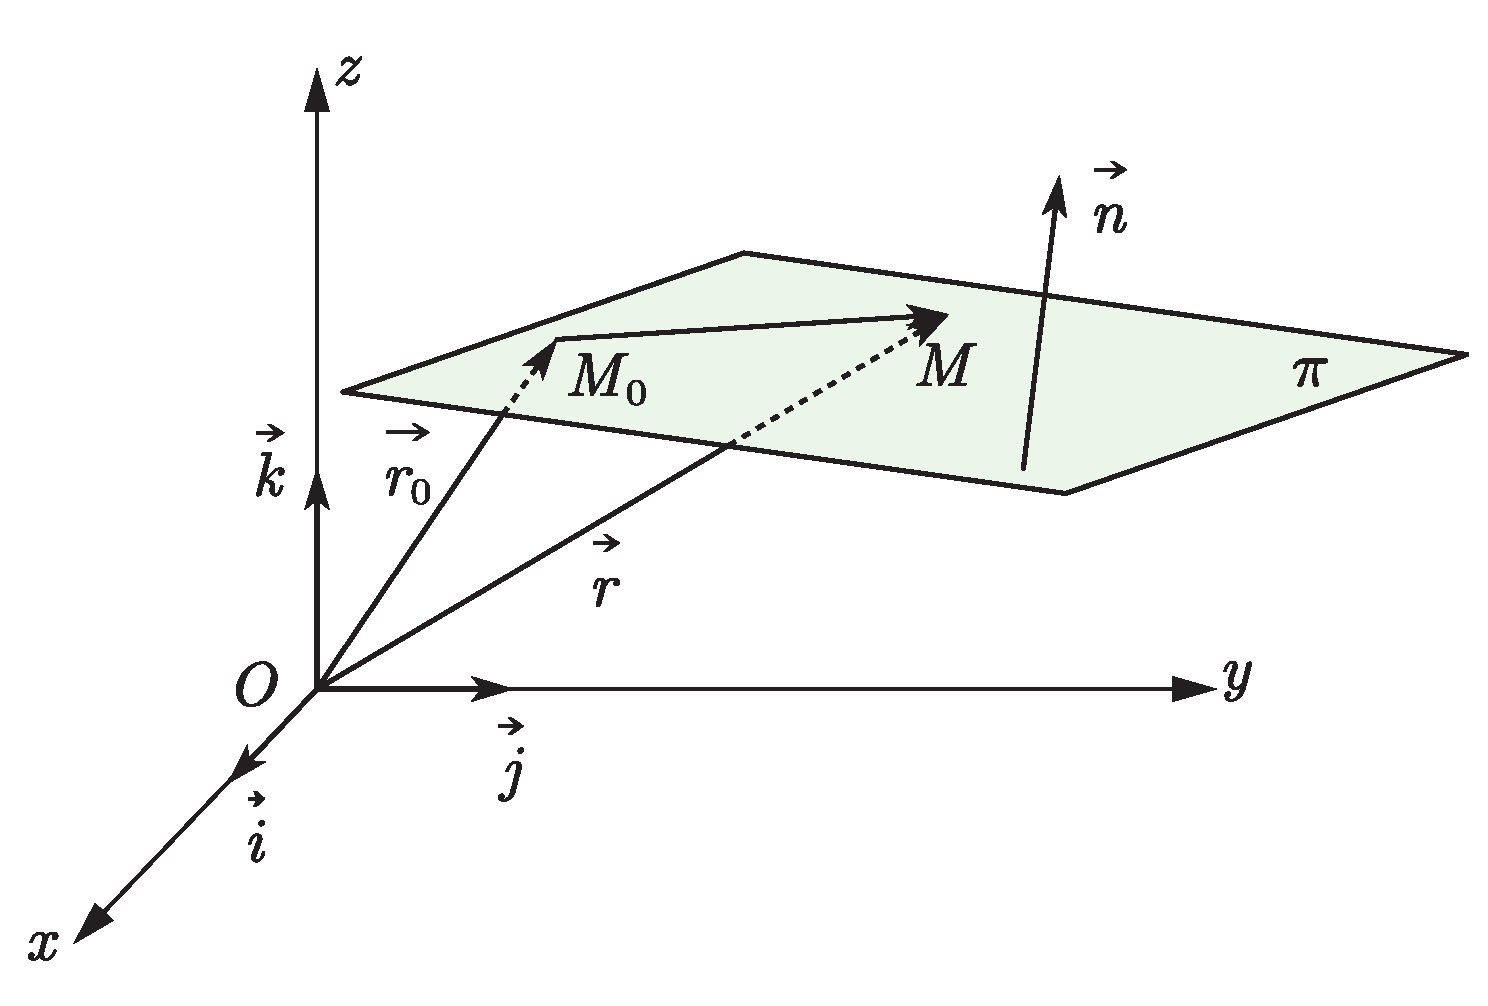
\includegraphics[width=0.9\linewidth]{picture/C-2/2.1/DFS.eps}
				%\caption{fig1}
				\label{DFS}
			\end{minipage}%
		}%
		\subfigure[向量式法式方程]{
			\begin{minipage}[b]{0.5\linewidth}
				\centering 
				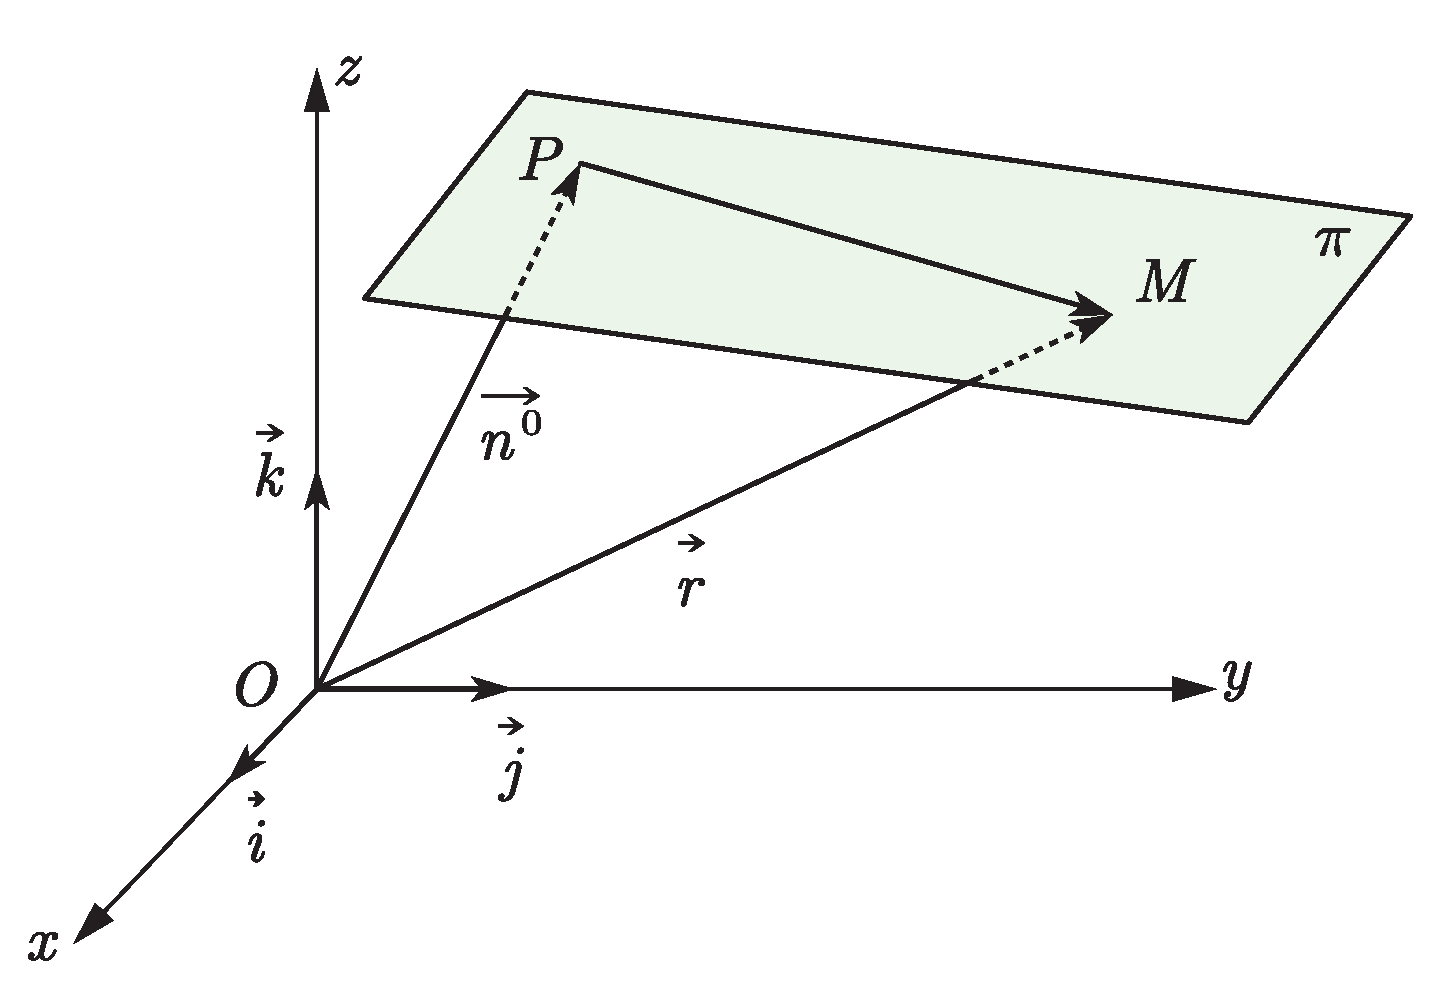
\includegraphics[width=0.9\linewidth]{picture/C-2/2.1/XLFS.eps}
				%\caption{fig2}
				\label{XLFS}
			\end{minipage}%
		}%
		\caption{直角坐标系平面方程}
	\end{figure}
	\label{平面的向量式法式方程}
	\item  {\color{dy}\large 向量式法式方程}\index{PMFC@平面方程!XLSFSFC@向量式法式方程}
	\begin{enumerate}[]
		\item 已知:{\color{dl}一个定点}:$P(x_0,y_0,z_0),$且{\color{dl}$\ \overrightarrow{OP}$垂直于平面$\pi $}.如图\ref{XLFS}.
		\item 原理:法向量的性质,取$\overrightarrow{OP}$的单位向量$\overrightarrow{n^0}$,那么向量$\overrightarrow{n^0}$是平面的单位法向量. 
		\item 表达式:设$M$的位置矢量分别是$\overrightarrow{r}$,$\left|\overrightarrow{OP} \right| =p$,则$\overrightarrow{OP} =p\overrightarrow{n^0}.$
		\begin{equation}
		\pi :\overrightarrow{n^0}\cdot \left(\overrightarrow{r}-p\overrightarrow{n^0} \right) =\overrightarrow{n^0}\cdot \overrightarrow{r}-p=0.
		\end{equation}
		\qquad 设$\overrightarrow{n^0}=\left(\cos \alpha ,\cos \beta ,\cos \gamma \right) $,其中$\alpha , \beta , \gamma$是向量$\overrightarrow{n^0}$的方向角,那么上式可以表示成\\
		{\color{dy}坐标式法式方程}:\index{PMFC@平面方程!ZBSFSFC@坐标式法式方程}
		\begin{equation}
		x\,\cos \alpha +y\,\cos \beta +z\,\cos \gamma-p=0.
		\end{equation}
	\end{enumerate}
	{\color{dy}法向量的方向规定}\\
	\hspace*{0.7cm} 如果点$P$是原点向平面$\pi $所引垂线的垂足,且法向量取单位法向量$\overrightarrow{n^0}$,那么
	\begin{enumerate}[(1)]
		\setlength{\itemindent}{3em}
		\setlength{\topsep}{0.01em}
		\setlength{\itemsep}{0.01em}
		\item 当平面不过原点时,规定$\overrightarrow{n^0}$正向与$\overrightarrow{OP}$相同,即{\color{dl}由原点指向平面};
		\item 当平面过原点时,$\overrightarrow{n^0}$正向在垂直于平面的两个方向中{\color{dl}任选一个}即可.
	\end{enumerate}
	{\color{dy}法式方程的特点}\\
	\hspace*{0.7cm} 平面的坐标式法式方程也是一种一般方程,但它满足两个条件:
	\begin{enumerate}[(1)]
		\setlength{\itemindent}{3em}
		\setlength{\topsep}{0.01em}
		\setlength{\itemsep}{0.01em}
		\item 一次项系数的平方和等于1;
		\item 常数项$-p \le 0$.
	\end{enumerate}
	{\color{dy}法式化因子}\\\index{PMFC@平面方程!XLSFSFC@向量式法式方程!FSHYZ@法式化因子}
	\hspace*{0.7cm} 要将直角坐标系下的一般方程
	\begin{equation*}
	Ax+By+Cz+D=0
	\end{equation*}
	化为法式方程,需要将法向量$\overrightarrow{n}=(A,B,C)$单位化,只要以
	\begin{equation}
	\lambda =\pm \frac{1}{|\overrightarrow{n}|}=\pm \frac{1}{\sqrt{A^2+B^2+C^2}}
	\end{equation}
	乘一般方程即可。$\lambda $的符号选取满足$\lambda D=-p \le 0.$即
	\begin{enumerate}[(1)]
		\setlength{\itemindent}{3em}
		\setlength{\topsep}{0.01em}
		\setlength{\itemsep}{0.01em}
		\item 当$D \neq 0$时,$\lambda $的符号与$D$相异;
		\item 当$D = 0$时,$\lambda $的符号可以任意选取其一.
	\end{enumerate}
	取定符号的因子$\lambda $称为平面的法式化因子.
\end{enumerate}
\section{特殊的平面方程}
对于平面一般式方程$Ax+By+Cz+D=0$,有
\begin{center}
	\begin{tabular}{|c|c|c|}
		\hline 
		条件&方程  &平面特点  \\ 
		\hline 
		$D=0$&$Ax+By+Cz=0$  & 通过原点 \\ 
		\hline 
		$A=0$&$By+Cz+D=0$  &\makecell [c]{\hspace*{0.5cm} 法向量$\overrightarrow{n}=(0,B,C)$  垂直于$x$轴,\hspace*{0.5cm} \\ \hspace*{0.5cm} 该平面平行(或包含)于$x$轴\hspace*{0.5cm} } \\ 
		\hline 
		$B=0$&$Ax+Cz+D=0$  &\makecell [c]{\hspace*{0.5cm} 法向量$\overrightarrow{n}=(A,0,C)$  垂直于$y$轴,\hspace*{0.5cm}  \\ \hspace*{0.5cm} 该平面平行(或包含)于$y$轴\hspace*{0.5cm} } \\ 
		\hline 
		$C=0$&$Ax+By+D=0$  &\makecell [c]{\hspace*{0.5cm} 法向量$\overrightarrow{n}=(A,B,0)$  垂直于$z$轴,\hspace*{0.5cm} \\ \hspace*{0.5cm} 该平面平行(或包含)于$z$轴\hspace*{0.5cm} } \\ 
		\hline 
		$A=B=0$& $\displaystyle Cz+D=0  (z=-\frac{D}{C})$ & \makecell [c]{\hspace*{0.5cm} 法向量$\overrightarrow{n}=(0,0,C)$  垂直于$x,y$轴,\hspace*{0.5cm} \\ \hspace*{0.5cm} 该平面平行(或重合)于$xOy$平面\hspace*{0.5cm} } \\ 
		\hline 
		$B=C=0$& $\displaystyle Ax+D=0 (x=-\frac{D}{A})$ & \makecell [c]{\hspace*{0.5cm} 法向量$\overrightarrow{n}=(A,0,0)$  垂直于$y,z$轴,\hspace*{0.5cm}  \\ \hspace*{0.5cm} 该平面平行(或重合)于$yOz$平面\hspace*{0.5cm} } \\ 
		\hline 
		$A=B=0$& $\displaystyle By+D=0 (z=-\frac{D}{B})$ & \makecell [c]{\hspace*{0.5cm} 法向量$\overrightarrow{n}=(0,B,0)$  垂直于$x,z$轴,\hspace*{0.5cm} \\ \hspace*{0.5cm} 该平面平行(或重合)于$xOz$平面\hspace*{0.5cm} } \\ 
		\hline 
	\end{tabular} 
\end{center}


\section{直线的方程}
\subsection{确定直线的条件}
\begin{enumerate}[$\bullet$]
	\setlength{\itemindent}{3em}
	\setlength{\topsep}{0.01em}
	\setlength{\itemsep}{0.01em}
	\item 过一定点可以作唯一直线平行于一定直线 .如图\ref{ZX1}.
	\item 两点可以确定一条直线.如图\ref{ZX2}.
	\item 任意一条直线可以视为两相交平面的交线.如图\ref{ZX3}.
\end{enumerate}
\begin{figure}[h]
	\subfigure[点和平行直线]{
		\begin{minipage}[b]{0.3\linewidth}
			\centering
			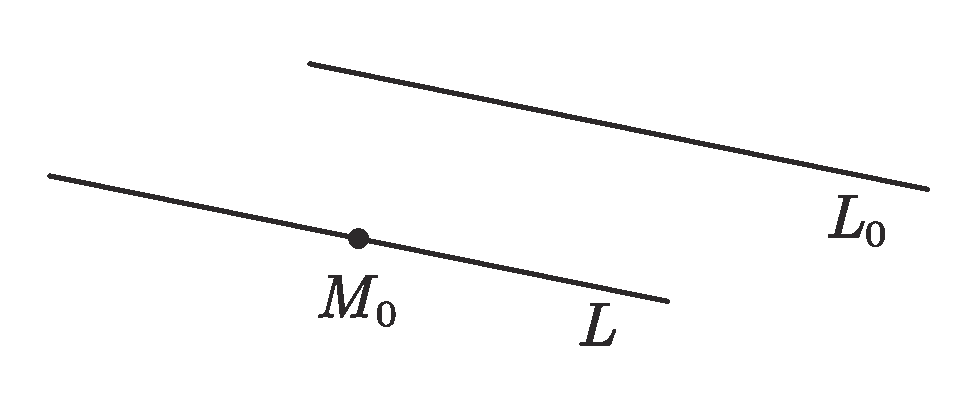
\includegraphics[width=0.9\linewidth]{picture/C-2/2.3/ZX1.pdf}
			\label{ZX1}
		\end{minipage}
	}
	\subfigure[两个不重合点]{
		\begin{minipage}[b]{0.3\linewidth}
			\centering
			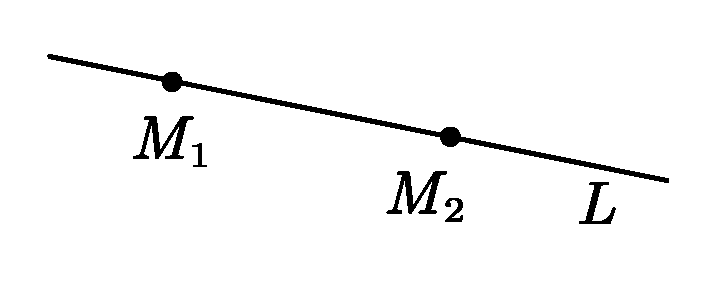
\includegraphics[width=0.9\linewidth]{picture/C-2/2.3/ZX2.pdf}
			\label{ZX2}
		\end{minipage}
	}
	\subfigure[两个相交平面]{
		\begin{minipage}[b]{0.4\linewidth}
			\centering
			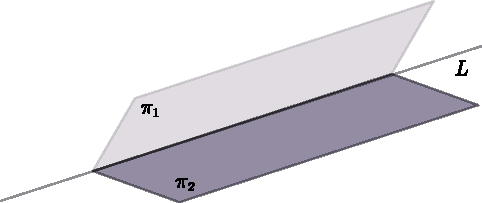
\includegraphics[width=0.9\linewidth]{picture/C-2/2.3/ZX3.pdf}
			\label{ZX3}
		\end{minipage}
	}
	\caption{确定直线的条件}
\end{figure}
\subsection{直线的通用方程}\index{ZXFC@直线方程}
\begin{enumerate}[\large1.]
	\item {\color{dy}\large 参数方程}\label{直线的参数方程}\index{ZXFC@直线方程!CSFC@参数方程}
	\begin{enumerate}[]
		\item 已知:{\color{dl}一点}:$M_0(x_0,y_0,z_0)$和{\color{dl}直线的方向向量}:$\overrightarrow{v}=(m,n,p)$.如图\ref{ZSCSFC}.
		\item 原理:过一定点可以作唯一直线平行于一定直线,直线上的所有向量都与该方平行.即
		$$\overrightarrow{M_0M}=t\overrightarrow{v}.$$
		\item 表达式:
		\begin{equation}
		L: \begin{cases}
		x=x_0+mt,\\
		y=y_0+nt,\\
		z=z_0+pt.
		\end{cases}(-\infty<t<+\infty).
		\end{equation}
		\item 特点:1.直线方程只含一个自由参数,通常说直线是一维的. \\
		2.直线可以看作匀速运动的质点轨迹,其中$\overrightarrow{v}$是速度,$t$是时间 .
	\end{enumerate}
	\begin{figure}[h]
		\subfigure[参数方程/点向式方程]{
			\begin{minipage}[b]{0.5\linewidth}
				\centering
				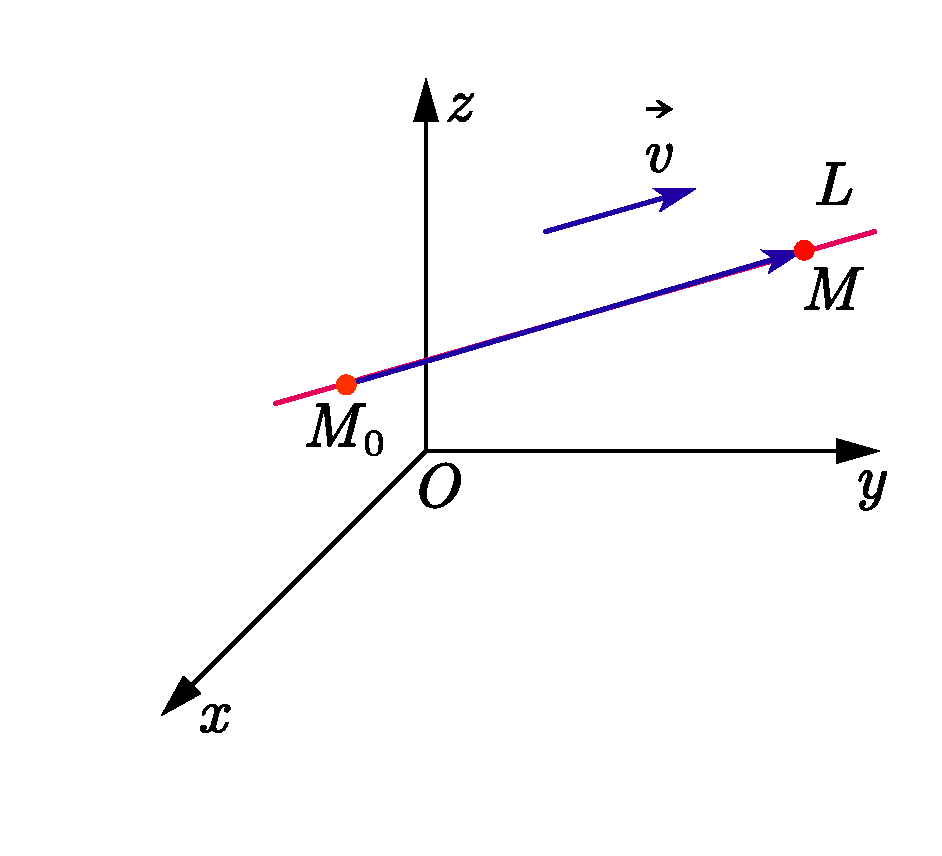
\includegraphics[width=0.9\linewidth]{picture/C-2/2.3/ZXCSFC.pdf}
				\label{ZSCSFC}
			\end{minipage}
		}
		\subfigure[向量式方程]{
			\begin{minipage}[b]{0.5\linewidth}
				\centering
				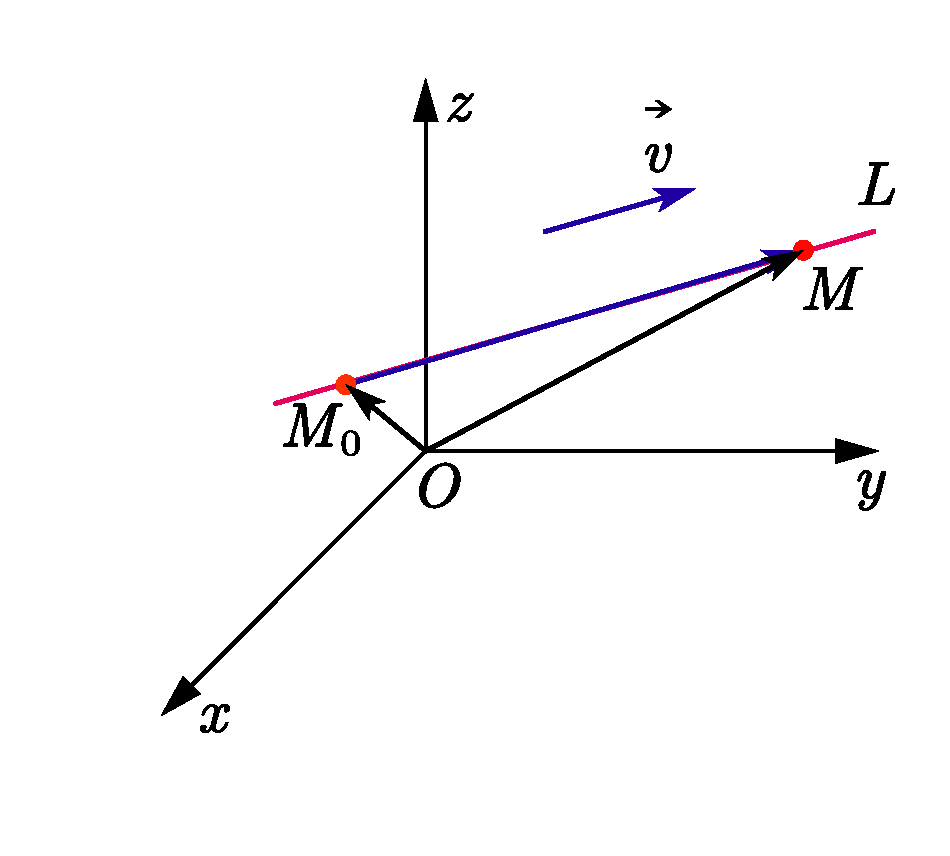
\includegraphics[width=0.9\linewidth]{picture/C-2/2.3/ZXXLSFC.pdf}
				\label{ZSXLSFC}
			\end{minipage}
		}
		\caption{直线的方程\uppercase\expandafter{\romannumeral1}}
	\end{figure}
	\item {\color{dy}\large 向量式方程}\index{ZXFC@直线方程!XLSFC@向量式方程}
	\begin{enumerate}[]
		\item 已知:{\color{dl}一点}:$M_0(x_0,y_0,z_0)$和{\color{dl}直线的方向向量}:$\overrightarrow{v}=(m,n,p)$.如图\ref{ZSXLSFC}.
		\item 原理:过一定点可以作唯一直线平行于一定直线,直线上的所有向量都与该方平行.即
		$$\overrightarrow{M_0M}=\overrightarrow{OM}-\overrightarrow{OM_0}=\overrightarrow{r}-\overrightarrow{r_0}=t\overrightarrow{v}.$$
		\item 表达式:
		\begin{equation}
		\overrightarrow{r}=\overrightarrow{r_0}+t\overrightarrow{v}
		\end{equation}
	\end{enumerate}
	\item {\color{dy}\large 点向式方程}\label{点向式方程}\index{ZXFC@直线方程!DXSFC@点向式方程}
	\begin{enumerate}[]
		\item 已知:{\color{dl}一点}:$M_0(x_0,y_0,z_0)$和{\color{dl}直线的方向向量}:$\overrightarrow{v}=(m,n,p)$.如图\ref{ZSCSFC}.
		\item 原理:$\overrightarrow{M_0M}$与方向向量$\overrightarrow{v}$平行.可以表示成
		$$\overrightarrow{M_0M}\times\overrightarrow{v}=\overrightarrow{0},\qquad  \overrightarrow{M_0M}=t\overrightarrow{v}.$$
		\item 表达式:
		\begin{equation}
		L: \frac{x-x_0}{m}=\frac{y-y_0}{n}=\frac{z-z_0}{p}
		\end{equation}
		\item 特点:点向式方程又称为{\color{dy}标准式方程}或{\color{dy}对称式方程}.
	\end{enumerate}
	\begin{figure}[h]
		\subfigure[两点式方程]{
			\begin{minipage}[b]{0.5\linewidth}
				\centering
				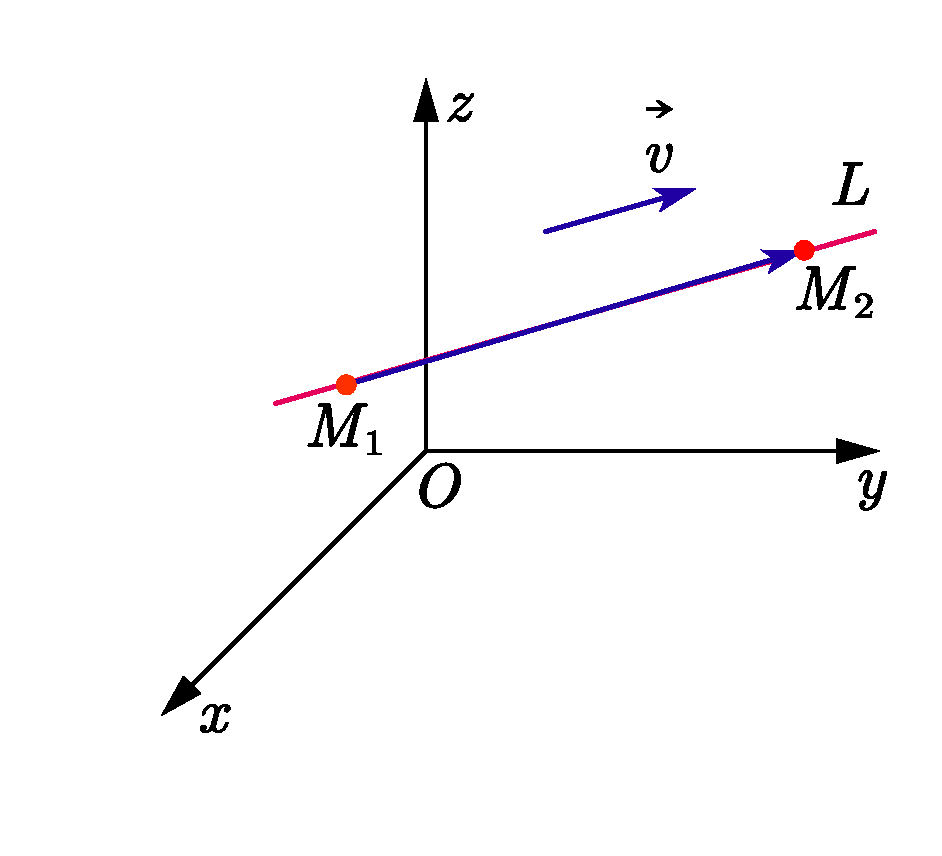
\includegraphics[width=0.9\linewidth]{picture/C-2/2.3/ZXLDSFC.pdf}
				\label{ZSLDSFC}
			\end{minipage}
		}
		\subfigure[一般式方程]{
			\begin{minipage}[b]{0.5\linewidth}
				\centering
				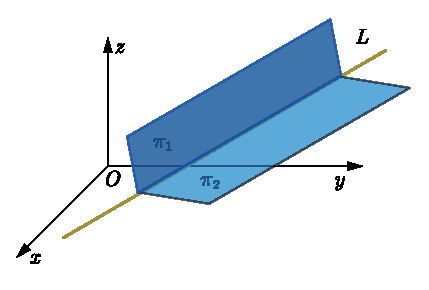
\includegraphics[width=0.9\linewidth]{picture/C-2/2.3/ZXYBFC.eps}
				\label{ZSYBFC}
			\end{minipage}
		}
		\caption{直线的方程\uppercase\expandafter{\romannumeral2}}
	\end{figure}
	\item  {\color{dy}\large 两点式方程}\label{两点式方程}\index{ZXFC@直线方程!LDSFC@两点式方程}
	\begin{enumerate}[]
		\item 已知:{\color{dl}不重合的两点}:$M_1(x_1,y_1,z_1),M_2(x_2,y_2,z_2)$.如图\ref{ZSLDSFC}.
		\item 原理:两点确定一条直线.本质上与点向式相同,即一个点$M_1(x_1,y_1,z_1)$和方向向量$\overrightarrow{v}=\overrightarrow{M_1M_2}$.
		\item 表达式:
		\begin{equation}
		L: \frac{x-x_1}{x_2-x_1}=\frac{y-y_1}{y_2-y_1}=\frac{z-z_1}{z_2-z_1}
		\end{equation}
	\end{enumerate}
	\newpage 
	\item  {\color{dy}\large 一般式方程}\index{ZXFC@直线方程!YBSFC@一般式方程}
	\begin{enumerate}[]
		\item 已知:{\color{dl}相交的两个平面}如图\ref{ZSYBFC}.
		\begin{equation*}
		\begin{cases}
		\pi_1:A_1x+B_1y+C_1z+D_1=0,\\
		\pi_2:A_2x+B_2y+C_2z+D_2=0.
		\end{cases}
		\end{equation*}
		\item 原理:任意一条直线可以视为两相交平面的交线.即联立两个平面方程.
		\item 表达式:
		\begin{equation}
		L: \begin{cases}
		\pi_1:A_1x+B_1y+C_1z+D_1=0,\\
		\pi_2:A_2x+B_2y+C_2z+D_2=0.
		\end{cases}
		\end{equation}
	\end{enumerate}
	\item  {\color{dy}\large 一般式方程转换为点向式方程}
	\begin{enumerate}[]
		\item 已知:{\color{dl}相交的两个平面}如图\ref{ZSYBFC}.
		\begin{equation*}
		\begin{cases}
		\pi_1:A_1x+B_1y+C_1z+D_1=0,\\
		\pi_2:A_2x+B_2y+C_2z+D_2=0.
		\end{cases}
		\end{equation*}
		\item 原理:直线与两个平面的法向量都垂直.叉乘后的向量与原来两个向量均垂直.
		\item 表达式:
		\begin{equation}
		\overrightarrow{v}=\overrightarrow{n_1}\times\overrightarrow{n_2}=
		\begin{array}{|ccc|}
		\overrightarrow{i} &\overrightarrow{j}  &\overrightarrow{k}  \\ 
		A_1 & B_1 & C_1 \\ 
		A_2 & B_2 & C_2
		\end{array} 
		\end{equation}
		再在两平面的交线上取一点$M_0(x_0,y_0,z_0)$即可.
	\end{enumerate}
\end{enumerate}


\section{线性图形的位置关系}
\subsection{平面与平面的位置关系}
\ttheorem[平面与平面的位置关系]
\quad 在仿射坐标系下,设两平面的方程为:
\begin{equation*}
\begin{array}{c}
\pi_1:A_1x+B_1y+C_1z+D_1=0,\\
\pi_2:A_2x+B_2y+C_2z+D_2=0.
\end{array}
\end{equation*}
那么,
\begin{enumerate}[$\mathrm (1)$]
	\setlength{\itemindent}{3em}
	\setlength{\topsep}{0.01em}
	\setlength{\itemsep}{0.01em}
	\item $\pi _1$与$\pi_2$相交于一条直线的充要条件是$\overrightarrow{n_1} \nparallel \overrightarrow{n_2} \Leftrightarrow A_1:B_1:C_1\ne A_2:B_2:C_2$.
	\item  $\pi _1$与$\pi_2$平行的充要条件是$\overrightarrow{n_1}\parallel\overrightarrow{n_2},\pi_1 \ne \pi_2 \Leftrightarrow \displaystyle \frac{A_1}{A_2}=\frac{B_1}{B_2}=\frac{C_1}{C_2} \ne \frac{D_1}{D_2}$.
	\item  $\pi _1$与$\pi_2$重合的充要条件是$\pi_1 = \pi_2 \Leftrightarrow \displaystyle \frac{A_1}{A_2}=\frac{B_1}{B_2}=\frac{C_1}{C_2}= \frac{D_1}{D_2}$.
\end{enumerate}
{\color{dy}本质:平面是否平行,法向量是平面定位的重要参考.重不重合看点,平不平行看法向量.}

\subsection{直线与直线的位置关系}
\ttheorem[直线与直线的位置关系]
\quad 在仿射坐标系下,设两直线方向向量为$\overrightarrow{v_1}=(m_1,n_1,p_1),\overrightarrow{v_2}=(m_2,n_2,p_2)$,分别过定点$M_1(x_1,y_1,z_1),M_2(x_2,y_2,z_2)$,其方程分别为:
\begin{equation*}
\begin{array}{c}
\displaystyle L_1:\frac{x-x_1}{m_1}=\frac{y-y_1}{n_1}=\frac{z-z_1}{p_1},\\
\displaystyle L_2:\frac{x-x_2}{m_2}=\frac{y-y_2}{n_2}=\frac{z-z_2}{p_2}
\end{array}
\end{equation*}
那么,记
\begin{equation*}
\Delta =\left[ \overrightarrow{v_1} \quad \overrightarrow{v_2} \quad \overrightarrow{M_1M_2}\right] =
\begin{array}{|ccc|}
m_1 & n_1 & p_1 \\ 
m_2 & n_2 & p_2 \\ 
x_2-x_1 & y_2-y_1 & z_2-z_1
\end{array} 
\end{equation*}
\begin{enumerate}[$\mathrm (1)$]
	\setlength{\itemindent}{3em}
	\setlength{\topsep}{0.01em}
	\setlength{\itemsep}{0.01em}
	\item  $L _1$与$L_2$平行的充要条件是$L_1 \parallel L_2 \Leftrightarrow \overrightarrow{v_1} \parallel \overrightarrow{v_2} \nparallel \overrightarrow{M_1M_2} \Leftrightarrow \displaystyle \frac{m_1}{m_2}=\frac{n_1}{n_2}=\frac{p_1}{p_2} \,,L_1 \ne \lambda L_2$.
	\item  $L _1$与$L_2$重合的充要条件是$L_1 \parallel L_2 \Leftrightarrow \overrightarrow{v_1} \parallel \overrightarrow{v_2} \parallel \overrightarrow{M_1M_2} \Leftrightarrow \displaystyle \frac{m_1}{m_2}=\frac{n_1}{n_2}=\frac{p_1}{p_2} \,,L_1 =\lambda L_2$.
	\item  $L _1$与$L_2$相交的充要条件是$\overrightarrow{v_1} \nparallel \overrightarrow{v_2},$且$\overrightarrow{v_1},\overrightarrow{v_2},\overrightarrow{M_1M_2}$共面$\Leftrightarrow \Delta = 0,\overrightarrow{v_1} \nparallel \overrightarrow{v_2}.$
	\item  $L _1$与$L_2$异面的充要条件是$\overrightarrow{v_1},\overrightarrow{v_2},\overrightarrow{M_1M_2}$不共面$\Leftrightarrow \Delta \ne  0.$
\end{enumerate}



\subsection{直线与平面的位置关系}
\ttheorem[直线与平面的位置关系]
\quad 在{\color{dy}直角坐标系}下,设法向量为$\overrightarrow{n}=(A,B,C)$的平面和过点$M_0(x_0,y_0,z_0)$且方向向量为$\overrightarrow{v}$的直线方程分别为:
\begin{equation*}
\begin{array}{c}
\pi:Ax+By+Cz+D=0,\\
\displaystyle L:\frac{x-x_0}{m}=\frac{y-y_0}{n}=\frac{z-z_0}{p}.
\end{array}
\end{equation*}
那么,
\begin{enumerate}[$\mathrm (1)$]
	\setlength{\itemindent}{3em}
	\setlength{\topsep}{0.01em}
	\setlength{\itemsep}{0.01em}
	\item  平面$\pi $与直线$L$平行的充要条件是$\overrightarrow{n} \perp \overrightarrow{v} \Leftrightarrow Am+Bn+Cp=0.$
	\item  平面$\pi $与直线$L$重合的充要条件是$\overrightarrow{n}  \perp \overrightarrow{v}$且$M_0(x_0,y_0,z_0)$在平面$\pi $上$\Leftrightarrow Am+Bn+Cp=0,Ax_0+By_0+Cz_0+D=0.$
	\item  平面$\pi $与直线$L$相交的充要条件是$\overrightarrow{n}  \not \perp \overrightarrow{v} \Leftrightarrow Am+Bn+Cp \neq 0.$
	\item  特别地,平面$\pi $与直线$L$垂直的充要条件是$\overrightarrow{n} \parallel  \overrightarrow{v} \Leftrightarrow \displaystyle \frac{A}{m}=\frac{B}{n}=\frac{C}{p}.$
\end{enumerate}



\subsection{平面束方程}\index{PMSFC@平面束方程}
\tdefination[定线平面束]\index{PMSFC@平面束方程!DXPMS@定线平面束}
过一条定直线的所有平面的集合称为{\color{dy}平面束方程},过直线
\begin{equation*}
L:
\begin{cases}
A_1x+B_1y+C_1z+D_1=0\\
A_2x+B_2y+C_2z+D_2=0
\end{cases}
\end{equation*}
的平面束方程为
\begin{equation}
\pi:\mu \left( A_1x+B_1y+C_1z+D_1\right) +\lambda \left( A_2x+B_2y+C_2z+D_2\right)=0.\quad (-\infty \leq \lambda ,\mu \leq +\infty)
\end{equation}


\defination[平行平面束]\index{PMSFC@平面束方程!PXPMS@平行平面束}
平行于平面$\pi :Ax+By+Cz+D=0$所有平面的集合称为{\color{dy}平行平面束方程},即表示为
\begin{equation}
Ax+By+Cz+D‘=0\quad (D' \neq D)
\end{equation}



\section{线性图形的距离}
\subsection{点到直线的距离}
\ttheorem[点到直线的距离]
在{\color{dy}直角坐标系}中,点$M(x,y,z)$到过定点$M_0(x_0,y_0,z_0)$,且方向向量为$\overrightarrow{v}=(m,n,p)$的直线
\begin{equation*}
L: \frac{x-x_0}{m}=\frac{y-y_0}{n}=\frac{z-z_0}{p}
\end{equation*}
的距离为:
\begin{equation}
d=\frac{|\overrightarrow{MM_0} \times \overrightarrow{v}|}{\left| \overrightarrow{v}\right| }.
\end{equation}


\subsection{离差}
\tdefination[离差]
\quad 如果从点$N$向平面$\pi $引垂线,垂足为点$M$,那么向量$\overrightarrow{MN}$在平面$\pi $上单位向量$\overrightarrow{n^0}$的射影叫做点$N$到平面$\pi $上的{\color{dy}离差},\index{LC@离差}记为:$\delta =\mathrm{Prj}_{\overrightarrow{n^0}}\overrightarrow{MN}.$

\noindent {\color{dy}离差的几何意义} 
\begin{enumerate}
	\item {\color{dy}\textbf{方向}}\quad 当点$N$位于平面$\pi $的单位法向量$\overrightarrow{n^0}$所指向的一侧时,离差$\delta >0$(即$\overrightarrow{MN}$与$\overrightarrow{n^0}$同向)\\
	当点$N$位于平面$\pi $的单位法向量$\overrightarrow{n^0}$所指向的另一侧时,离差$\delta <0$(即$\overrightarrow{MN}$与$\overrightarrow{n^0}$反向).
	\item {\color{dy}\textbf{大小}}\quad 离差的绝对值$|\delta| $等于点$N$到平面$\pi $的距离$d$.
\end{enumerate}
\theorem[点与平面的位置关系]
\quad 设平面$\pi $的向量法式方程为
\begin{equation*}
\pi :\overrightarrow{n^0}\cdot \overrightarrow{r}-p=0.\quad \mbox{或} \quad  x\cos \alpha+y\cos \beta +z\cos \gamma-p=0 
\end{equation*}
其中,$\overrightarrow{n^0}$为平面$\pi $的单位法向量,$p$为原点到平面$\pi $的距离.\\
\quad 则点$M_0(x_0,y_0,z)$关于平面$\pi $的离差为
\begin{equation}
\delta =x_0\cos \alpha+y_0\cos \beta +z_0\cos \gamma-p=\frac{Ax_0+By_0+Cz_0+D}{\sqrt{A^2+B^2+C^2}}
\end{equation}
因此,我们可以借此判断点$M_0$在平面$\pi $的位置(假设$\overrightarrow{n^0}$指向平面$\pi $上方):
\begin{enumerate}[$\mathrm (1)$]
	\setlength{\itemindent}{3em}
	\setlength{\topsep}{0.01em}
	\setlength{\itemsep}{0.01em}
	\item $Ax_0+By_0+Cz_0+D>0 \Longleftrightarrow $点$M_0$在平面$\pi $上方;
	\item $Ax_0+By_0+Cz_0+D=0 \Longleftrightarrow $点$M_0$在平面$\pi $内;
	\item $Ax_0+By_0+Cz_0+D<0 \Longleftrightarrow $点$M_0$在平面$\pi $下方.
\end{enumerate}



\subsection{点到平面的距离}
\ttheorem[点到平面的距离]
\quad 在{\color{dy}直角坐标系}中,点$P_1(x_1,y_1,z_1)$到平面\\
\begin{minipage}{0.6\linewidth}
	$$\pi : Ax+By+Cz+D=0$$
	的距离为:
	\begin{equation}
	d=\frac{\left| Ax_1+By_1+Cz_1+D\right| }{\sqrt{A^2+B^2+C^2}}
	\end{equation}
\end{minipage}
\hfill
\begin{minipage}{0.4\linewidth}
	\centering
	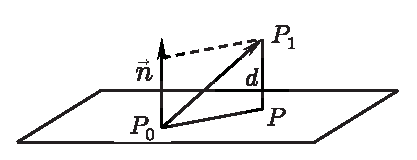
\includegraphics[scale=1]{picture/C-2/2.5/point.eps}
\end{minipage}
证明思路:利用向量在平面法向量上的投影. 如图,
$$d=\frac{\left| \overrightarrow{P_0P_1} \cdot \overrightarrow{n}\right| }{\left| \overrightarrow{n}\right| }=\frac{|(Ax_1+By_1+Cz_1)-(Ax+By+Cz+D)+D|}{\sqrt{A^2+B^2+C^2}}=\frac{\left| Ax_1+By_1+Cz_1+D\right| }{\sqrt{A^2+B^2+C^2}}$$



\subsection{平面到平面的距离}
\ttheorem[平面到平面的距离]
\quad 两平行平面$\pi _1:Ax+By+Cz+D_1=0,\pi _2:Ax+By+Cz+D_2=0(D_1 \neq D_2)$的距离为:
\begin{equation}
d=\frac{\left| D_1-D_2\right| }{\sqrt{A^2+B^2+C^2}}
\end{equation}

证明思路:在其中一个平面上任取一点即变成点到平面的距离求解。
\subsection{两直线的公垂线}
\tdefination[公垂线段]
分别与两条异面直线$l_1,l_2$垂直相交的直线$l$叫做$l_1,l_2$的公垂线\index{GCX@公垂线},两垂足的连线称为公垂线段\index{GCXD@公垂线段}。


\theorem[两直线的公垂线]
\quad 两异面直线$l_1,l_2$分别过点$M_1(x_1,y_1,z_1),M_2(x_2,y_,2z_2)$,且方向向量分别为$\overrightarrow{v_1}=(m_1,n_1,p_1),\overrightarrow{v_2}=(m_2,n_2,p_2)$.即
\begin{equation*}
\begin{array}{c}
\displaystyle l_1:\frac{x-x_1}{m_1}=\frac{y-y_1}{n_1}=\frac{z-z_1}{p_1},\\
\displaystyle l_2:\frac{x-x_2}{m_2}=\frac{y-y_2}{n_2}=\frac{z-z_2}{p_2}
\end{array}
\end{equation*}
\qquad 那么公垂线的方向向量可取$\overrightarrow{v_1} \times \overrightarrow{v_2} \neq 0$,设公垂线上一点$M(x,y,z)$,那么由$\overrightarrow{M_1M},\overrightarrow{v_1},\overrightarrow{v}$可确定一个平面$\pi_1$。同理,$\overrightarrow{M_2M},\overrightarrow{v_2},\overrightarrow{v}$可确定一个平面$\pi_2$,而公垂线就是这两个平面的交线,即
\begin{equation}
\begin{cases}
\left( \overrightarrow{r_M}-\overrightarrow{r_{M_1}}\,,\,\overrightarrow{v_1}\,,\,\overrightarrow{v}\right) =0\\
\left( \overrightarrow{r_M}-\overrightarrow{r_{M_2}}\,,\,\overrightarrow{v_2}\,,\,\overrightarrow{v}\right) =0
\end{cases}
\end{equation}
用坐标表示,得
\begin{equation}
\begin{cases}
\,
\begin{array}{|ccc|}
x-x_1 &y-y_1  &z-z_1  \\ 
m_1&n_1  &p_1  \\ 
m&n  &p 
\end{array}=0\\ 
\quad \\
\,
\begin{array}{|ccc|}
x-x_2 &y-y_2  &z-z_2  \\ 
m_2&n_2  &p_2  \\ 
m&n  &p 
\end{array}=0
\end{cases}
\end{equation}


\subsection{直线到直线的距离}
\begin{enumerate}[\large1.]
	\item {\color{dy}\large 异面直线情形}
	
	\enbelowtheorem[异面直线的距离]
	\quad 设两条异面直线$l_1,l_2$分别过点$M_1,M_2$,方向向量分别为$\overrightarrow{v_1},\overrightarrow{v_2}$,则$l_1,l_2$之间的距离为
	\begin{equation}
	d=\frac{\left| \left( \overrightarrow{M_1M_2}\,,\,\overrightarrow{v_1}\,,\,\overrightarrow{v_2}\right) \right| }{\left| \overrightarrow{v_1} \times \overrightarrow{v_2}\right|}.
	\end{equation}
	证明思路:两条异面直线$l_1,l_2$之间的距离$d$可以理解为以$\overrightarrow{M_1M_2}\,,\,\overrightarrow{v_1}\,,\,\overrightarrow{v_2}$为棱的平行六面体的体积(利用\hyperref[混合积的几何意义]{\color{超链接}混合积的几何意义}\footnote{总结的超链接均用{\color{超链接}此颜色}表示})除以$\overrightarrow{v_1}\,,\,\overrightarrow{v_2}$为邻边的平行四边形的面积(利用\hyperref[外积的几何意义]{\color{超链接}叉乘的几何意义}).
	
	
	\item {\color{dy}\large 平行直线情形}
	\begin{enumerate}[]
		\item 在任意一条直线上取一点,转换成点到直线的问题解决。
	\end{enumerate}
\end{enumerate}

\section{线性图形的夹角}
\subsection{平面与平面的夹角}
\quad 两个{\color{dy}平面的夹角}是指两个平面变成两个相邻的二面角中中任一个. 其中一个等于两个法向量的夹角.如图\ref{平面与平面的夹角}.\\

\theorem[平面与平面的夹角]
\quad 设在{\color{dy}直角坐标系}中,两个平面$\pi_1 \pi_2$的方程分别为:
\begin{equation*}
\begin{array}{c}
\pi_1:A_1x+B_1y+C_1z+D_1=0,\\
\pi_2:A_2x+B_2y+C_2z+D_2=0.
\end{array}
\end{equation*}
则$\pi_1$与$ \pi_2$的一个夹角 $\theta $满足:
\begin{equation}
\cos \theta =\frac{\overrightarrow{n_1}\cdot \overrightarrow{n_2}}{\left| \overrightarrow{n_1}\right| \left|  \overrightarrow{n_2}\right| }
=\frac{A_1A_2+B_1B_2+C_1C_2}{\sqrt{A_1^2+B_1^2+C_1^2}\cdot \sqrt{A_2^2+B_2^2+C_2^2}}
\end{equation}
那么由此可以知道两个平面$\pi_1 \pi_2$垂直的充要条件为:
\begin{equation}
A_1A_2+B_1B_2+C_1C_2=0.
\end{equation}


\begin{figure}[h]
	\subfigure[平面与平面的夹角]{
		\begin{minipage}[b]{0.4\linewidth}
			\centering
			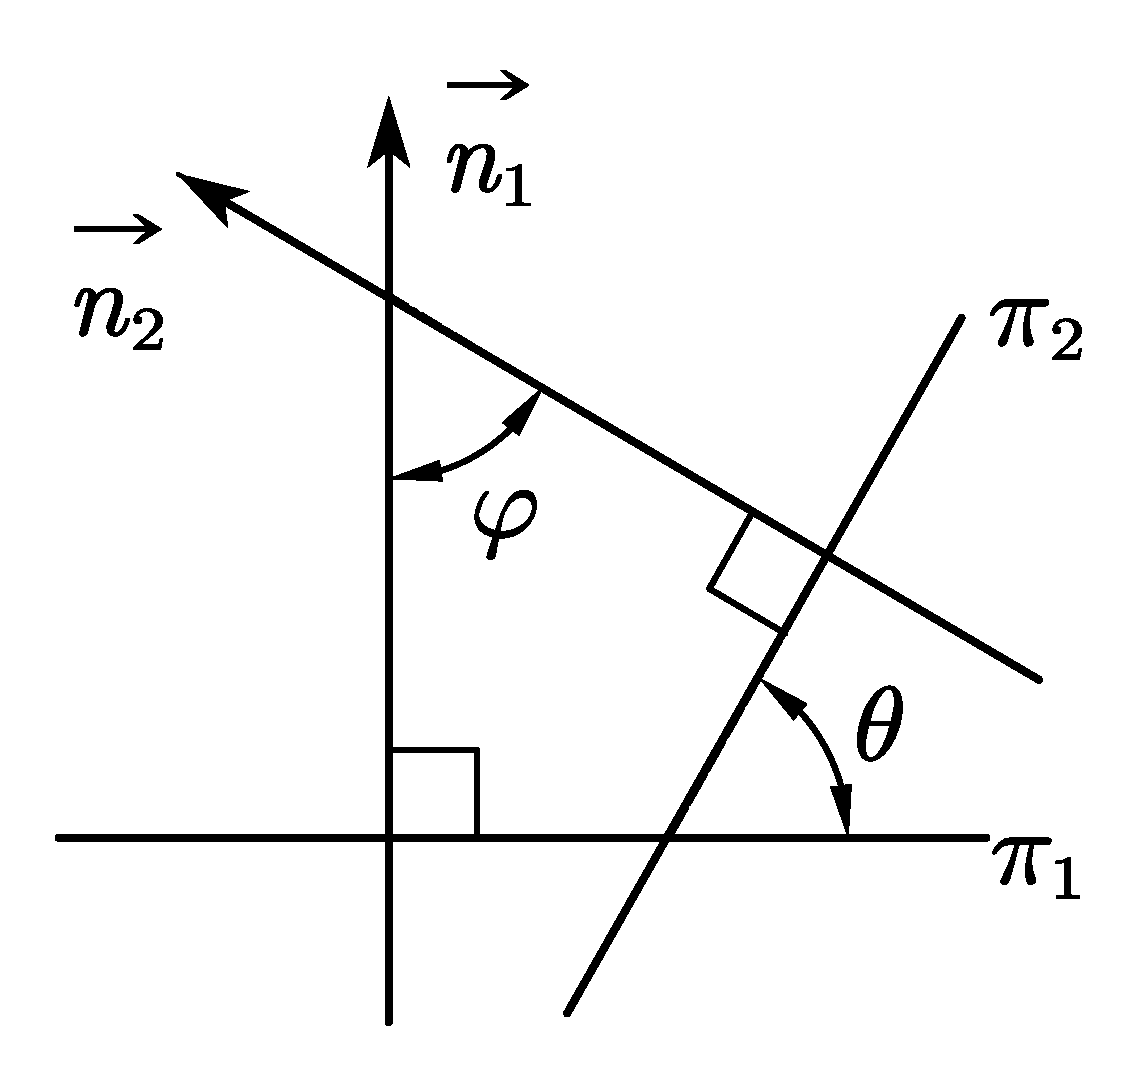
\includegraphics[width=0.7\linewidth]{picture/C-2/2.6/JJ1.pdf}
			\label{平面与平面的夹角}
		\end{minipage}
	}
	\subfigure[两直线夹角]{
		\begin{minipage}[b]{0.2\linewidth}
			\centering
			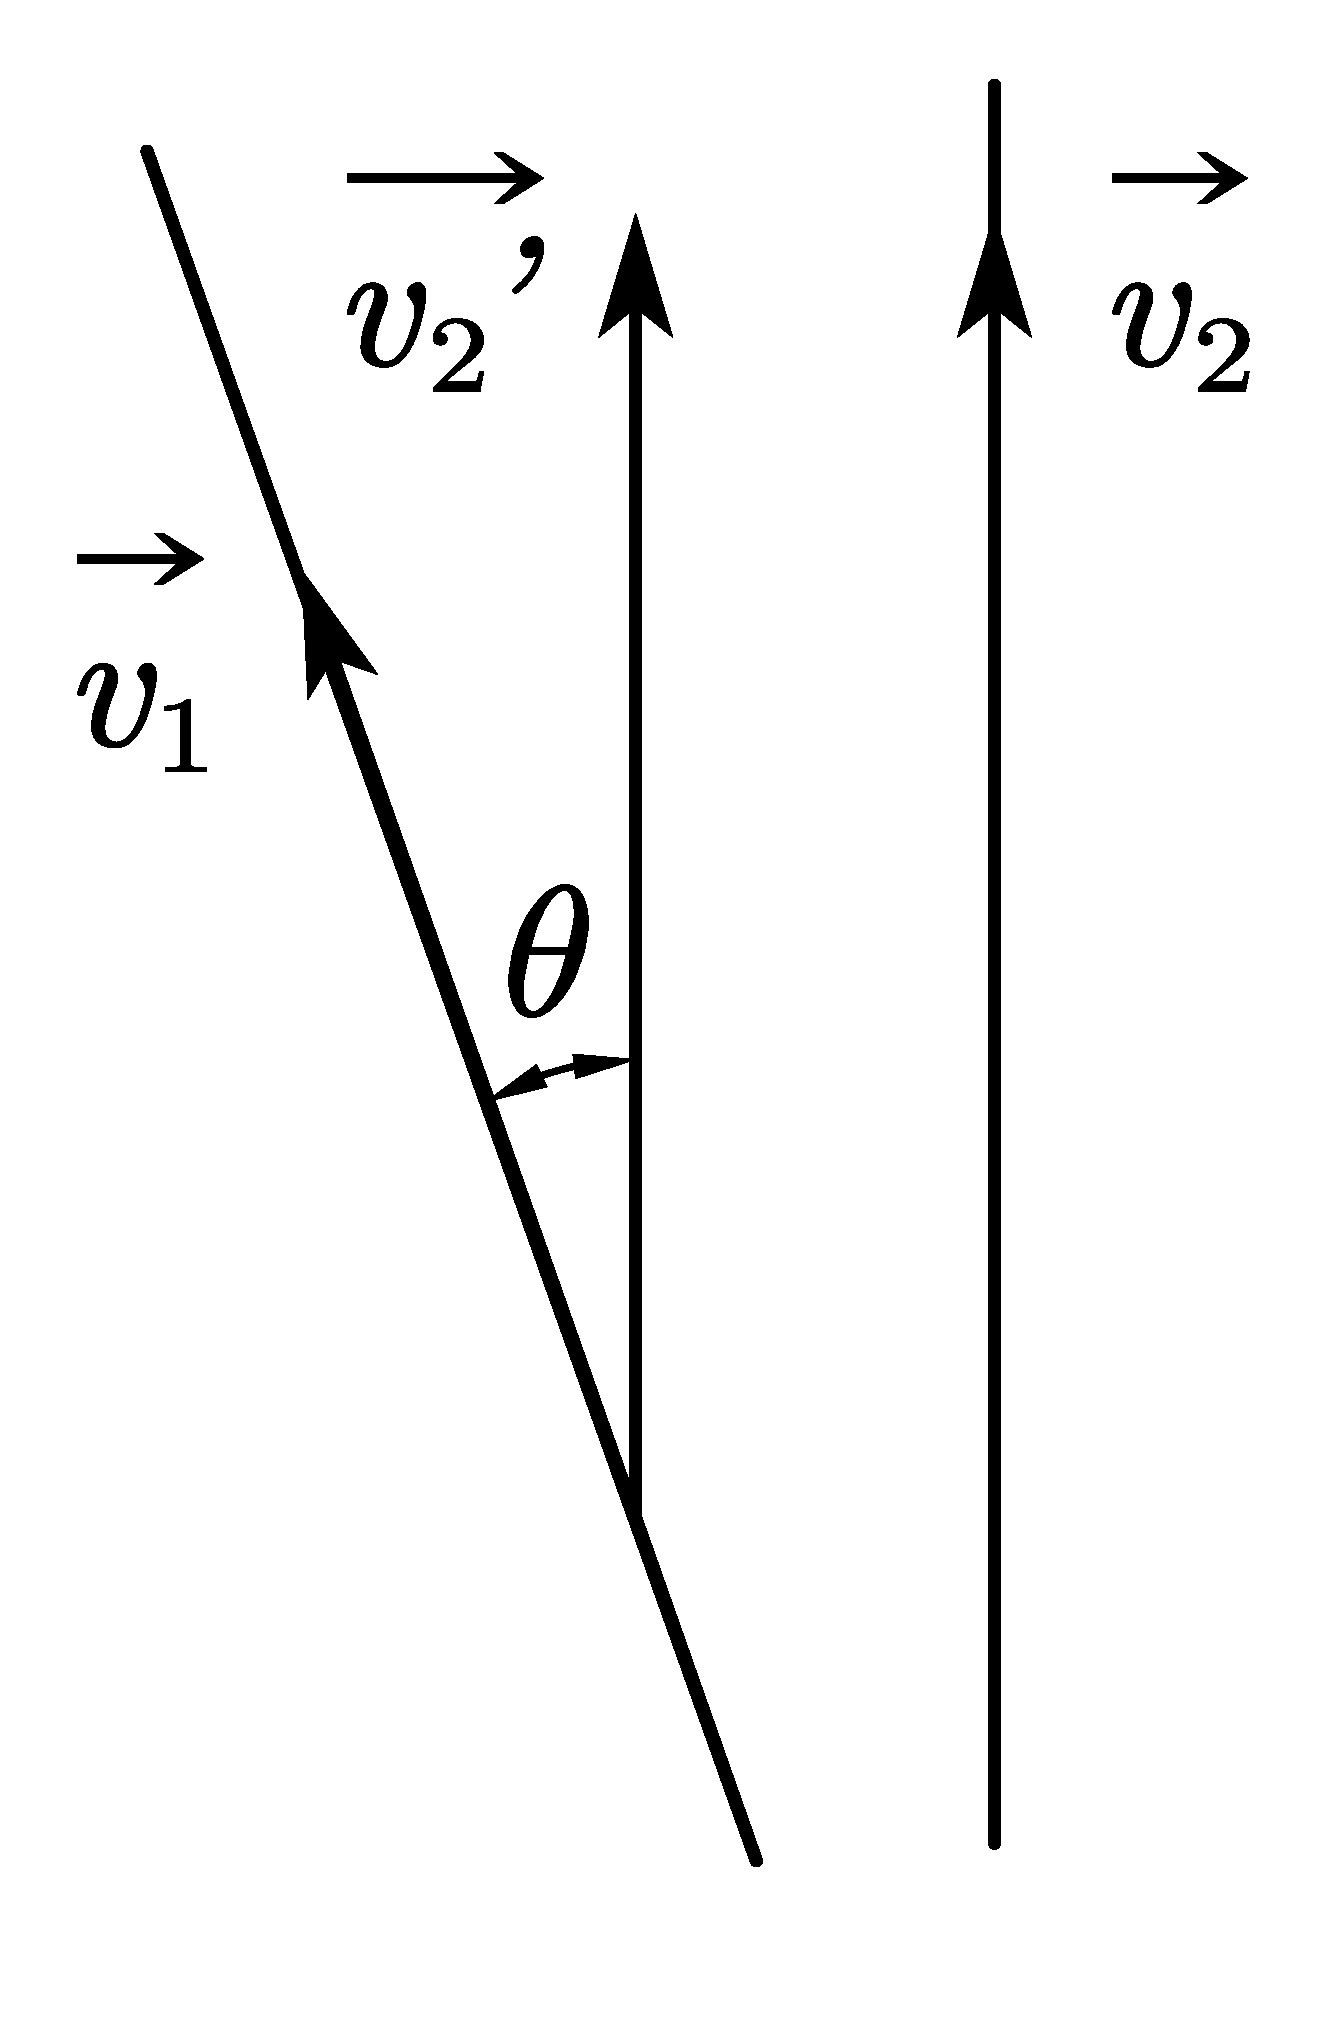
\includegraphics[width=0.8\linewidth]{picture/C-2/2.6/JJ2.pdf}
			\label{两直线的夹角}
		\end{minipage}
	}
	\subfigure[直线和平面的夹角]{
		\begin{minipage}[b]{0.4\linewidth}
			\centering
			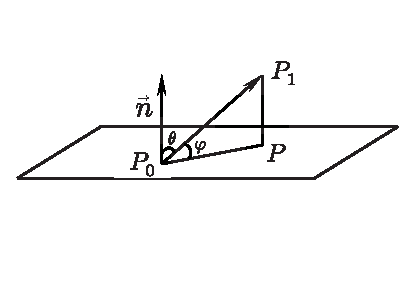
\includegraphics[width=0.9\linewidth]{picture/C-2/2.6/JJ3.eps}
			\label{直线和平面的夹角}
		\end{minipage}
	}
						\caption{线性图形的夹角}
\end{figure}
\subsection{两直线的夹角}
\quad 两条{\color{dy}直线的夹角}是指它们的方向向量的夹角或其补角.如图\ref{两直线的夹角}.

\theorem[两直线的夹角]
\quad 设在{\color{dy}直角坐标系}中,两条直线$L_1,L_2$的方向向量分别为:$\overrightarrow{v_1}=(m_1,n_1,p_1),\overrightarrow{v_2}=(m_2,n_2,p_2).$则$L_1,L_2$的夹角为$\left\langle \overrightarrow{v_1},\overrightarrow{v_2}\right\rangle $或$\pi -\left\langle \overrightarrow{v_1},\overrightarrow{v_2}\right\rangle ,$则
\begin{equation}
\begin{split}
\cos \left\langle L_1,L_2\right\rangle &=\pm \cos \left\langle \overrightarrow{v_1},\overrightarrow{v_2}\right\rangle =\pm \frac{\overrightarrow{v_1}\cdot \overrightarrow{v_2}}{|\overrightarrow{v_1}|\cdot |\overrightarrow{v_2}|}\\
&=\pm \frac{m_1m_2+n_1n_2+p_1p_2}{\sqrt{m_1^2+n_1^2+p_1^2}\cdot \sqrt{m_2^2+n_2^2+p_2^2}}
\end{split}
\end{equation}


特别地,直线$L_1,L_2$垂直的充分必要条件是:
\begin{equation}
m_1m_2+n_1n_2+p_1p_2=0
\end{equation}

\subsection{直线与平面的夹角}
\quad 当直线和平面垂直时,{\color{dy}直线与平面的夹角}是指这条直线和它在平面上的垂直射影所构成的{\color{dy2}锐角}。当直线垂直于平面时,规定{\color{dy}直线与平面的夹角}为{\color{dy2}直角}。如图\ref{直线和平面的夹角}.

\theorem[直线与平面的夹角]
\quad 设在{\color{dy}直角坐标系}中,直线$L$的方向向量为:$\overrightarrow{v}=(m,n,p).$平面$\pi $的法向量$\overrightarrow{n}=(X,Y,Z)$,设直线$L$与平面$\pi $的夹角为$\varphi \in \displaystyle \left[ 0,\frac{\pi }{2} \right],\left\langle \overrightarrow{v},\overrightarrow{n}\right\rangle =\theta \in \displaystyle \left[ 0,\pi  \right]$,则由图\ref{直线和平面的夹角}.可知:
$$\varphi =\left| \frac{\pi }{2}-\theta \right| $$
即
\begin{equation}
\begin{split}
\sin \varphi &=|\cos \theta |=\frac{|\overrightarrow{n} \cdot \overrightarrow{v} |}{|\overrightarrow{n}| \cdot |\overrightarrow{v}|}\\
&=\frac{\left| mX+nY+pZ\right| }{\sqrt{X^2+Y^2+Z^2}\,\cdot \,\sqrt{m^2+n^2+p^2}}.
\end{split}
\end{equation} 
